\chapter{Security of IP networks}

\begin{figure}[h]
    \centering
    \includegraphics[page = 2,trim = 0.7cm 2.2cm 0.7cm 4cm, clip, width = 0.55\textwidth]{\slides}
    \caption{Remote access via dial-up lines}
\end{figure}

%\paragraph*{Remote access via dial-up lines}
The first point regarding the security of IP networks involves \ul{controlling who can access the networks}.
In the past, it was primarily used for residential users who utilized a modem to connect to a telephone line (switched network).
This process involved transforming bits into sound and having equivalent equipment on the ISP side, which would accept the telephone call and convert it into network packets.
To facilitate this, devices known as \textbf{NAS} (\textit{Network Access Server}) were employed.
NAS had the responsibility of \underline{authenticating users}, \underline{performing access control}, and subsequently \underline{providing users with access} to the IP network - typically the internet, but in some cases also allowing access to a company's internal network from home.
Nowadays, this system is no longer widely used, at least in Western countries, although some countries still rely on it.


\begin{figure}[h]
    \centering
    \includegraphics[page = 3,trim = 0.7cm 2.2cm 0.7cm 3.7cm, clip, width = 0.55\textwidth]{\slides}
    \caption{Network access (modern way)}
\end{figure}

%\paragraph*{Network access (modern way)}
Today, it is possible to access the Internet in different ways, which basically depends on the device.
For example, a smartphone typically uses technologies such as 3G, 4G, or 5G to connect to the base station, which runs an \textbf{authentication protocol} with the \textbf{AAA server} to check if the user is authorized for an internet connection.
It is also possible to use Wi-Fi to connect to access points, which provide the translation from a wireless to a wired network and can again verify access.
Alternatively, there could be a home gateway, which provides access to the Internet using both Ethernet and Wi-Fi (only if properly authenticated).
In all these scenarios, authentication is always required before permitting traffic from a specific user.
Therefore, there is a difference between the \textit{local branch} / \textit{last mile}, \textit{border element}, and \textit{the core network}.



\section{Authentication of PPP channels}
There is a need to authenticate a user before enabling network transmission. The authentication process begins when someone attempts to connect, and at this point, the physical layer (Layer 1) for physical transmissions is already available. Since we are working at a logical level, Layer 2 (data layer connectivity) is also accessible.

On top of data layer connectivity, a protocol specific to transporting data is usually running. Typically, this protocol is \textbf{PPP} (\textit{Point-to-Point Protocol}), designed to \textbf{encapsulate network packets} such as Layer 3 (e.g., IP) and \textbf{carry them over a point-to-point link}. This PPP link can be a physical connection like an ISDN line or a telephone network; alternatively, it can be a virtual layer, as is the case when starting from a home gateway with access to ADSL using PPPoE (PPP over Ethernet) to transport packets between the home gateway and the provider.

Moreover, PPP is utilized to carry packets within virtualized Layer 3 connections with a specific and somewhat complex\footnote{The professor described it as "horrible"} protocol named L2TP (Layer 2 Tunnel Protocol). L2TP is a Layer 2 encapsulated inside UDP/IP (which is Layer 4), which deviates from the normal behaviors of a network.

Regardless, once PPP is enabled, numerous virtual point-to-point connections extend from the device to an access point. PPP activation occurs in three steps:

\begin{enumerate}
    \item \textbf{LCP (Link Control Protocol):} Establishes the ability to transmit data, and can also negotiate authentication protocols and algorithms.
    \item \textbf{Authentication (optional; PAP, CHAP, or EAP):} Performs user authentication.
    \item \textbf{L3 encapsulation:} Handles Layer 3 encapsulation via various \textbf{NCP}s (Network Control Protocols), such as IPCP (IP Control Protocol).
\end{enumerate}




\subsection{Authentication of a network access}
There are three methods to authenticate network access over PPP:

\begin{itemize}
    \item \textbf{PAP (Password Authentication Protocol):} This is the oldest method; in this case, the user sends the username and password in clear over the PPP channel. If someone is sniffing the channel, they can acquire the password.

    \item \textbf{CHAP (Challenge Handshake Authentication Protocol):} It uses a symmetric challenge-response based on the user's password. In this case, the password cannot be copied, but the channel is not protected. Instead of inventing other protocols tied to a specific authentication mechanism, a generalization has been made by introducing EAP.

    \item \textbf{EAP (Extensible Authentication Protocol):} It is a authentication framework that does not implement any specific method. The authentication method is external; for example, challenge-response, OTP, or TLS can be used.
\end{itemize}

Nowadays, PAP and CHAP should never be used, while EAP is the most widely adopted method for authenticating network access.

\subsection{LCP Authentication - Protocol
    Configuration Option}
If the Protocol Configuration Option in LCP Authentication exists, it includes several components:

\begin{itemize}
    \item \textbf{Type (8-bit):} Denotes the option type.
    \item \textbf{Length (8-bit):} Represents the length of the option in bytes.
    \item \textbf{Authentication Protocol (16-bit):} Specifies the protocol identifier.
    \item \textbf{[ Algorithm (8-bit) ]:} Optional field for algorithm identifier, required when a protocol supports various algorithms.

          For PAP (Password Authentication Protocol):
          \begin{itemize}
              \item \textbf{Type:} 3
              \item \textbf{Length:} 4
              \item \textbf{Protocol:} \texttt{0xC023}
          \end{itemize}

          For CHAP (Challenge Handshake Authentication Protocol):
          \begin{itemize}
              \item \textbf{Type:} 3
              \item \textbf{Length:} 5
              \item \textbf{Protocol:} \texttt{0xC223}
              \item \textbf{Algorithm:} 5 (for MD5)
          \end{itemize}
\end{itemize}


% NOTE: PAP and CHAP sections were added in 2023/24
\subsubsection{PAP}
\textbf{PAP}, or \textit{Password Authentication Protocol}, is defined in RFC-1334 "PPP Authentication Protocols" (Oct 1992). This RFC also introduces the initial version of CHAP.

In PAP, the user-id and password are transmitted in clear text between the Peer and the Authenticator, posing a significant security risk. Authentication occurs only once when the channel is created, making it a potentially vulnerable method. Due to the clear transmission of sensitive information, PAP is considered very dangerous and is not recommended for secure network communication.

\paragraph{PAP: 2-way Handshake Protocol}
PAP employs a 2-way handshake protocol involving communication between the Peer and the Authenticator.

\begin{itemize}
    \item ($Peer \rightarrow Authenticator$) \texttt{Authenticate-Request} ($code=1$)
          \begin{itemize}
              \item Code (8-bit) + Identifier (8-bit) + Length (16-bit)
              \item Peer-ID Length (8-bit) + Peer-ID (0-255B)
              \item Passwd-Length (8-bit) + Password (0-255B)
          \end{itemize}
    \item ($Authenticator \rightarrow Peer$) \texttt{Authenticate-Response} ($code= 2, 3$)
          \begin{itemize}
              \item Code (8-bit) + Identifier (8-bit) + Length (16-bit)
              \item Msg-Length (8-bit) + Message (0-255B)
              \item Code=2 (ACK), Code=3 (NAK)
          \end{itemize}
\end{itemize}

An identifier is essential for correlating the \texttt{Authenticate-Request} with its corresponding \texttt{Authenticate-Response}. Given the potential loss of either loss of either request or response, it becomes imperative for the Authenticator to accommodate multiple requests. Therefore, to mitigate the risk of lost messages, the Authenticator \textbf{MUST} allow for the submission of multiple \texttt{Authenticate-Request} or \texttt{Authenticate-Response} messages.
This identifier is also pivotal in preventing replay attacks. Without it, an adversary could intercept and replay the message, potentially granting unauthorized access.



\subsubsection{CHAP}
\textbf{CHAP}, or \textit{Challenge Handshake Authentication Protocol}, is defined in RFC-1994 "PPP Challenge Handshake Authentication Protocol (CHAP)" (Aug 1996). It introduces a symmetric challenge (password-based) authentication mechanism.

In CHAP, the initial challenge is compulsory and occurs at channel creation. The authentication request can optionally be repeated, with a different challenge, during transmission. The decision to repeat the authentication request is taken by the Network Access Server (NAS). It's important to note that the challenge MUST be a nonce.

For systems supporting both PAP and CHAP, the Authenticators must offer CHAP as the preferred authentication method.

\paragraph{CHAP: 3-way Handshake Protocol}
CHAP employs a 3-way handshake protocol involving communication between the Authenticator and the Peer.
\underline{After the link is established}:

\begin{itemize}
    \item ($Authenticator \rightarrow Peer$) \texttt{Challenge} ($code=1$)
          \begin{itemize}
              \item Code (8-bit) + Identifier (8-bit) + Length (16-bit)
              \item Challenge-Size (8-bit) + Challenge-Value (0-255B)
          \end{itemize}
    \item ($Peer \rightarrow Authenticator$) \texttt{Response} ($code=2$)
          \begin{itemize}
              \item Code (8-bit) + Identifier (8-bit) + Length (16-bit)
              \item Response-Size (8-bit) + Response-Value (0-255B)
          \end{itemize}
    \item ($Authenticator \rightarrow Peer$) \texttt{Result} ($code= 3$ Success, $4$ Failure)
          \begin{itemize}
              \item Code (8-bit) + Identifier (8-bit) + Length (16-bit)
          \end{itemize}
\end{itemize}

\textit{Response-Value} is calculated using \texttt{md5(Identifier || pwd || Challenge-Value)} (in the version specified in 1996). The server checks the response by comparing it with its own calculation of the expected hash value. If the values match, the authentication is acknowledged; otherwise, the connection is usually terminated.

The identifier is crucial for correlating the Request and Response. In case of lost \texttt{Challenge} or \texttt{Response}, the Authenticator \textbf{MUST} resend the Challenge until the retry limit is reached.



\subparagraph*{Packet Loss in PPP Implementation}
One interesting point to consider is the idea that challenges or responses could be lost in a PPP (point-to-point protocol). You might wonder why, especially when we have a direct connection between two peers using an Ethernet cable or Wi-Fi. Usually, in such direct connections, we expect very little or no loss of information.

The confusion arises due to the varied ways PPP can be used. We mentioned earlier that PPP can operate on different types of transport, including a virtual setup within UDP. Here's the catch: UDP, unlike other more reliable protocols, doesn't ensure that your data reaches its destination every time. Moreover, UDP is built on top of IP, which also doesn't guarantee that your information will be reliably delivered.

This becomes apparent when we consider how PPP packets are implemented in real-world situations. In some cases, instead of sticking to the logical layering (PPP being at layer 2), PPP packets may be placed inside layer 4 due to certain implementation choices. This might seem like a strange decision, but it happens. As a result, even though you might think a direct point-to-point connection is rock-solid, these implementation choices could lead to some data loss. So, when designing such protocols, it's crucial to account for all possible scenarios, even the ones that might seem unlikely at first.


\paragraph{MS-CHAP}
MS-CHAP, or Microsoft PPP CHAP Extensions, is a set of protocols developed by Microsoft to enhance the functionality of the Challenge Handshake Authentication Protocol (CHAP) in PPP connections\footnote{"The usual approach from Microsoft, in which they take something standard and make it non-standard".}.


\begin{itemize}
    \item \textbf{MS-CHAPv1:}
          \begin{itemize}
              \item RFC 2433 "Microsoft PPP CHAP Extensions" (October 1998).
              \item Initially included but later discontinued by Microsoft starting with Windows Vista.
          \end{itemize}

    \item \textbf{MS-CHAPv2:}
          \begin{itemize}
              \item RFC 2759 "Microsoft PPP CHAP Extensions, v2" (January 2000).
              \item Continued the evolution of MS-CHAP, dropped by Microsoft starting with Windows 11 22H2.
          \end{itemize}
\end{itemize}

LCP negotiates the CHAP algorithm, with \texttt{0x80} for MS-CHAPv1 and \texttt{0x81} for MS-CHAPv2, using option 3 (Authentication Protocol).

MS-CHAP is a Microsoft-specific implementation of CHAP concepts.
Despite its origin, MS-CHAP is supported by many other vendors, including CISCO.


\subparagraph{MS-CHAP: Extensions over CHAP}
MS-CHAP extends the principles of CHAP but operates as a distinct protocol with unique features.

\begin{itemize}
    \item \textbf{Common Features (v1 and v2):}
          \begin{itemize}
              \item Authenticator-controlled password change.
              \item Authenticator-controlled authentication retry.
              \item Specific failure codes.
          \end{itemize}

    \item \textbf{MS-CHAPv2 Mutual Authentication:}
          \begin{itemize}
              \item Achieved by piggybacking a peer challenge on the Response packet.
              \item Includes an authenticator response on the Success packet.
          \end{itemize}
\end{itemize}

In order to implement this protocol, each peer must know the plaintext password or an MD4 hash of the password. Note: This approach is not compatible with most password storage formats.


\begin{figure}[H]
    \centering
    \includegraphics[page = 13,trim = 0.5cm 2.2cm .5cm 4cm, clip, width = .70\textwidth]{\slides}
    \caption{The MS-CHAPv2 protocol}
\end{figure}

\begin{figure}[H]
    \centering
    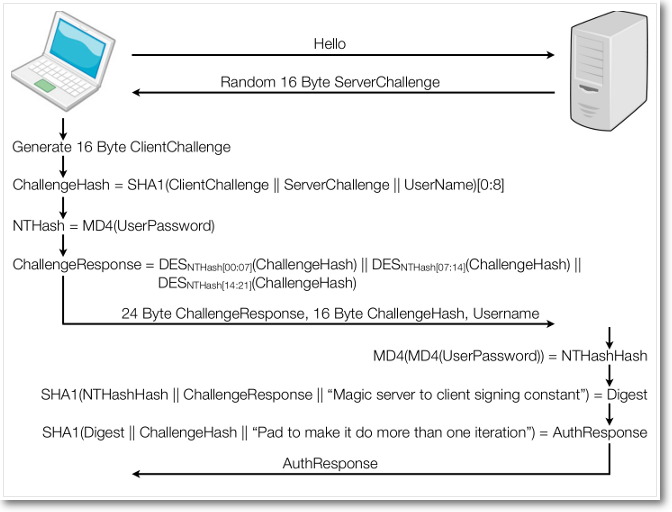
\includegraphics[width = .70\textwidth]{chapter4/MS-CHAPv2.png}
    \caption{MS-CHAPv2 - Another frame of reference. Please consider the professor's slide. Taken from\\
        \url{https://web.archive.org/web/20160316174007/https://www.cloudcracker.com/blog/2012/07/29/cracking-ms-chap-v2/}}
\end{figure}


\subparagraph{MS-CHAPv2: an attack}
MS-CHAPv2, once deemed a secure authentication protocol, is susceptible to a specific attack exploiting a known ciphertext-plaintext pair denoted as \(R\) and \(H\). The primary objective is to decipher the three keys, namely \(K_{0-6}\), \(K_{7-13}\), and \(K_{14-20}\). Directly employing a brute-force approach on the password is considered impractical due to the significant time involved. Alternatively, a brute-force attack on the keys poses a challenge, requiring approximately \(2^{56} + 2^{56} + 2^{56}\) operations.

However, it's crucial to note that \(K\) is only 128 bits (MD4 output), i.e., 16 bytes, and \(K_{14-20}\) has only two bytes (\(K_{14-15}\)) padded with zeros. To find \(K_{14-20}\), \(2^{16}\) operations are needed. The process involves \(2^{56}\) operations to find \(K_{0-6}\) and \(K_{7-13}\), followed by a comparison with \(R1\) and \(R2\). Utilizing a divide-and-conquer strategy reduces the effort to approximately \(2^{56}\) operations (less than 23 hours with DES FPGA).

\begin{figure}[H]
    \centering
    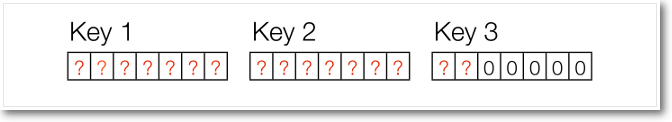
\includegraphics[width = .70\textwidth]{chapter4/MS-CHAPv2_attack1.png}
    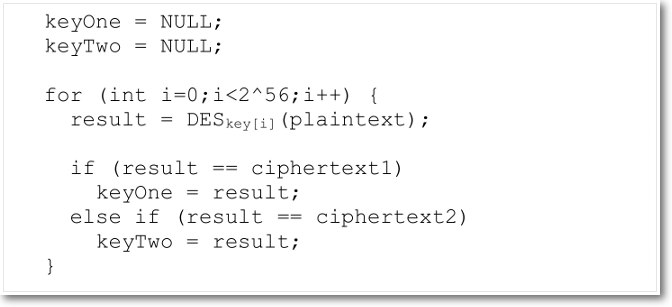
\includegraphics[width = .70\textwidth]{chapter4/MS-CHAPv2_attack2.png}
\end{figure}

In conclusion, MS-CHAPv2 should NEVER be used anymore and has been officially deprecated, including its removal in Windows 11 22H2.


\subsubsection{EAP}
EAP (\textit{Extensible Authentication Protocol}) is the PPP authentication mechanism  defined in RFC-3748, providing a \textbf{flexible Layer 2 (L2) authentication framework}. This L2 authentication occurs before accessing the internet, which operates at Layer 3 (L3). EAP supports various predefined authentication mechanisms, such as \textit{MD5-challenge} (symmetric and akin to CHAP), \textit{generic OTP}, and \textit{generic token card}.
Additional mechanisms, such as RFC-2716 "PPP EAP TLS authentication protocol" and RFC-3579 "RADIUS support for EAP," have been incorporated.

As EAP performs authentication before reaching L3, it requires its encapsulation protocol for transporting data, including usernames, challenges, or responses, over L2.

\begin{itemize}
    \item EAP introduces a small L3 protocol exclusively for its use, offering \textbf{independence from IP} and compatibility with diverse link layers (e.g., old PPP and 802.x).
    \item Due to the absence of L3, EAP \textbf{provides ACK/NAK} for packets but lacks windowing (as seen in TCP). EAP assumes that packets won't be reordered, a guarantee provided by PPP, but if EAP is utilized over virtual channels like UDP and raw IP, datagrams may arrive out of order, potentially disrupting EAP functionality.
    \item \textbf{Retransmission} is essential to ensure packet delivery, with a typical limit of 3 to 5 retransmission attempts; authentication fails if this limit is exceeded.
    \item EAP \textbf{does not handle fragmentation}, dependent on the MTU of the underlying L2 network. EAP methods must manage payloads exceeding the minimum EAP MTU.
\end{itemize}


When authentication fails in EAP, it does not necessarily indicate a failure in the authentication process; rather, it could be attributed to a network problem. When troubleshooting EAP, the expertise of a network specialist may be required to identify and address any issues causing the failure.

In EAP, the assumption is that \underline{the link is not inherently physically secure}, requiring each authentication method to ensure its security. Some EAP methods include:
\begin{itemize}
    \item \textbf{EAP-TLS (RFC-5216):}
    \item \textbf{EAP-MD5 (RFC-3748):} Symmetric challenge-response providing only EAP peer authentication without mutual authentication.
    \item \textbf{EAP-TTLS:} TLS tunneling that allows the operation of any method protected inside a secure TLS channel.
    \item \textbf{EAP-SRP (Secure Remote Password)}
    \item \textbf{GSS-API (includes Kerberos)}
    \item \textbf{AKA-SIM (RFC-4186, RFC-4187):} Subscriber Identity Module, the system used in mobile networks.
\end{itemize}

\begin{figure}[h]
    \centering
    \includegraphics[page = 18,trim = 1cm 2.2cm 1cm 4cm, clip, width = 0.55\textwidth]{\slides}
    \caption{EAP - architecture}
    \label{fig:eap-architecture}
\end{figure}

In Figure \ref*{fig:eap-architecture}, the general architecture of EAP is depicted. The lower part represents various L2 channels supported by EAP, including PPP, 802.3 (Ethernet), 802.5 (Token Ring), and 802.11 (Wi-Fi). EAP extends its authentication methods, such as TLS, AKA-SIM, and SRP authentication, to these specific networks independently of the L2 layer.

\section{Authentication for network access}
\begin{figure}[h]
    \centering
    \includegraphics[page = 19,trim = .5cm 3cm .5cm 5cm, clip, width = 0.55\textwidth]{\slides}
    \caption{Authentication for network access}
    \label{fig:eap-authentication}
\end{figure}

Authentication for network access operates as illustrated in the architecture in Figure \ref{fig:eap-authentication}. On the left, various communication links (modems, access points, or ADSL/Fiber) terminate at a device hosted by the ISP. These devices, designed to connect multiple users, are controlled by a NAS (Network Access Server), which receives requests from clients and determines the validity of the user. The NAS employs a protocol on the backend IP network local to the NAS and subsequently communicates with the centralized authentication server. This approach is necessary as ISPs have multiple points of presence with numerous NAS devices that must share consistent user information.

The authentication server possesses access to a database containing user credentials and configuration details for each user, based on the contract between the user and the ISP. The Authentication Server responds to the NAS with the user's authentication status (valid/invalid) and the configuration that the NAS must enforce on the user's traffic.

\paragraph{AAA}
NAS manufacturers claim that security needs three functions briefly named as AAA:
\begin{itemize}
    \item \textbf{Authentication:} entity's identity is authenticated based on credentials (e.g., password, OTP);
    \item \textbf{Authorization:} determining whether an entity is authorized to perform a given activity or gain access to the resources or services;
    \item \textbf{Accounting:} tracking network resource usage for audit support, capacity analysis, or cost billing.
\end{itemize}

The AS performs exactly these three functions talking with one or more NAS via one or more protocols.

\subparagraph{Network Authentication Protocols}
Basically, there are three protocols that AS (Authentication Server) and NAS can use to communicate:
\begin{itemize}
    \item \textbf{RADIUS:} It is the de-facto standard and the most widely used one, with a feature that allows it to act as a \underline{proxy towards other authentication systems}. It can serve as both an authentication system and use external AS.
    \item \textbf{DIAMETER:} This protocol is the evolution of RADIUS, emphasizing roaming among different ISPs. Since it is more modern, it pays better attention to security.
    \item \textbf{TACACS+ (TACACS, XTACACS):} A competitor of RADIUS, technically superior, but achieved lower acceptance due to being a \underline{proprietary solution} implemented only by Cisco with no public specification.
\end{itemize}


\subsection{RADIUS}\label{chap:radius}
RADIUS stands for \textbf{Remote Authentication Dial-In User Service}. It is a legacy protocol developed nearly 30 years ago, initially designed for Dial-In scenarios when users connected to an ISP using modems. Over time, RADIUS has evolved and \textbf{now supports authentication, authorization, and accounting (AAA)} to control network access for various types of ports:

\begin{itemize}
    \item \textbf{Physical ports} (analogical, ISDN, IEEE 802): RADIUS can be utilized for access control on Ethernet networks as well.
    \item \textbf{Virtual ports} (tunnel, wireless access): It enables centralized management of a network of access points.
\end{itemize}

RADIUS, as a concept, implements \textbf{centralized administration and accounting} to store information about resource usage. It operates as a \textbf{client-server protocol} \textit{between the NAS and AS}, utilizing \texttt{port 1812/UDP} for \textit{authentication} and \texttt{port 1813/UDP} for \textit{accounting}.
Since UDP is unreliable, each transmission of a RADIUS packet is subject to timeout. If no ACK is received after the \textit{timeout}, the same packet is \textit{retransmitted}, with a maximum number of attempts before declaring communication impossible.
RADIUS supports architectures with a main server and numerous \textit{secondary servers}, enhancing system performance, and resilience (also against DoS attacks).

\begin{itemize}
    \item RFC-2865 (Protocol): Specifies the RADIUS protocol for remote authentication and accounting.
    \item RFC-2866 (Accounting): Defines additional attributes and guidelines for RADIUS accounting.
    \item RFC-2867/2868 (Tunnel Accounting and Attributes): Describes extensions for handling tunnel attributes and accounting in RADIUS.
    \item RFC-2869 (Extensions): Provides extensions to RADIUS to support additional attributes.
    \item RFC-3579 (RADIUS Support for EAP): Outlines RADIUS support for the Extensible Authentication Protocol (EAP).
    \item RFC-3580 (Guidelines for 802.1X with RADIUS): Presents guidelines for using RADIUS with the IEEE 802.1X standard.
\end{itemize}

From the list above it is possible to see that from the basic protocol there have been a lot of extensions (also
the EAP support) and in particular it supports also 802.1X (Chapter \ref{chap:802.1x}) which is a network access control security
architecture.


\subsubsection{RADIUS proxy}
The \textbf{RADIUS server} may act as a \textbf{proxy} towards other authentication servers. In the depicted scenario (Figure \ref{fig:radius-proxy}), there are two NAS on the left, each sending an access request from users. RADIUS consults its \textit{local RADIUS DB} on the right and checks if, for example, "Barbara" is a valid registered user. If it receives an access request, perhaps from another NAS, in the form of an email address (although it is not an email address), such as alice@WIN.polito.it, it indicates that the user Alice is not registered in the local RADIUS DB. Instead, Alice is a user defined in the security domain WIN.polito.it to which the RADIUS server is associated somehow.

This implies that \textbf{RADIUS will act as a proxy for the \underline{authentication part}} and redirect the request to the Windows domain controller. The authorization/accounting could then be managed locally by the RADIUS server. RADIUS can also be associated with another domain, such as a UNIX NIS server.

\begin{figure}[h]
    \centering
    \includegraphics[page = 24,trim = 1cm 2.3cm 1cm 7cm, clip, width = 0.55\textwidth]{\slides}
    \caption{Radius proxy}
    \label{fig:radius-proxy}
\end{figure}


\subsubsection{RADIUS security functionalities}
RADIUS requires security functionalities due to various potential threats:

\begin{itemize}
    \item \textbf{Sniffing NAS Requests (if contains passwords):}\\
          This poses a \textit{confidentiality} problem, as sniffing a request containing a password in clear text could lead to unauthorized access. Even in scenarios where passwords are not sent in clear text (e.g., OTP systems), a privacy concern arises, as sniffing the traffic could reveal user actions without revealing the actual password. There are no issues with sniffing the response, as it only indicates the validity of the request.

    \item \textbf{Fake AS Response (to block valid or allow invalid user):}\\
          Attackers could exploit the UDP nature of RADIUS to provide faster responses than the legitimate server. The first received response is considered valid, allowing for potential denial-of-service (DoS) attacks to block valid users or provide positive responses to invalid ones. Authentication of responses is crucial in such cases.

    \item \textbf{Changing AS Response (Y → N or N → Y):} Unauthorized modification of responses from valid to invalid or vice versa is a possibility. Authentication and integrity checks for responses are necessary to mitigate this type of attack.

    \item \textbf{Replay of AS Response (if not properly tied to NAS req):}\\
          Replay attacks could occur if responses are not properly tied to specific requests. If a response is generic (e.g., only "valid" or "invalid"), attackers could replay a valid response to another user. To prevent this, responses should contain user identification (e.g., "Antonio Lioy, who connected at XX:XX time, is valid").

    \item \textbf{Passwords Enumeration (from fake NAS):}\\
          If an attacker gains access to the back-end network between the NAS and RADIUS server, they might create a fake NAS and send requests to the RADIUS server to enumerate passwords. Authentication from NAS requests is required to mitigate this risk.

    \item \textbf{DoS (many NAS requests from fake NAS):} \\
    An attacker with access to the back-end network could flood the RADIUS server with numerous requests, rendering it unavailable. \ul{NAS are configured with a list of various RADIUS servers}, and if a response delay occurs, the NAS assumes the server is busy and switches to the next one. The system's resistance to this attack is proportional to the number of secondary servers configured.
\end{itemize}


\subsubsection{RADIUS characteristics}
For \textbf{data protection}, RADIUS employs packet integrity and authentication via \textbf{keyed-MD5}:

\begin{itemize}
    \item The key is a shared secret between the NAS and the RADIUS Server, ensuring that inserting a fake NAS server into the network will result in the rejection of its requests.
    \item In cases where packets contain a password (e.g., if a user decides to use PAP and the password is sent in clear), the password is transmitted in an "encrypted" manner (not true encryption, but rather obfuscated using MD5, which is a digest algorithm, not an encryption algorithm): \( \text{{password}} \oplus \text{{md5}}(\text{{key}} + \text{{authenticator}}) \). This is padded with NULL bytes until a multiple of 128 bits is reached.
\end{itemize}

RADIUS supports various authentication methods (PAP, CHAP, token-card, and EAP). Cisco provides a free server for CryptoCard, and others also support SecurID. Importantly, RADIUS is an \textbf{extensible protocol} because each packet carries attributes described in TLV form \texttt{(attribute type - length - value)}. This allows the introduction of new types without breaking compatibility.


\vspace*{5mm}
\noindent
\begin{minipage}{0.5\textwidth}
  \centering
  \includegraphics[page = 28,trim = 3cm 3cm 3cm 2cm, clip, width = \linewidth]{\slides}
\end{minipage}
\hspace{0.05\textwidth}
\begin{minipage}{0.4\textwidth}

    The format of a RADIUS packet includes the following components:
    \begin{itemize}
        \item \texttt{Code} (8 bits)
        \item \texttt{Identifier} (8 bits)
        \item \texttt{Length} (16 bits)
        \item \texttt{Authenticator} (128 bits)
        \item \texttt{TLV} (Type-Length-Value) list of attributes
    \end{itemize}  
\end{minipage}

\vspace*{7mm}    
RADIUS supports various packet types, and some of them include:

\begin{itemize}
    \item \texttt{ACCESS-REQUEST:} Contains access credentials (e.g., username and password).
    \item \texttt{ACCESS-REJECT:} Access is denied (e.g., due to bad username/password).
    \item \texttt{ACCESS-CHALLENGE:} Requests additional information from the user (e.g., PIN, token code, secondary password).
    \item \texttt{ACCESS-ACCEPT (parameters):} Access is granted, and some network parameters are given (e.g., IP address, netmask, MTU, host, port, ...).
\end{itemize}


\paragraph*{RADIUS - authenticator}
Inside packets, the \texttt{authenticator} serves a \underline{dual purpose}: 
\begin{enumerate}
    \item in the \textit{server reply}, it provides \textit{authentication} and \textit{protection from replay};
    \item while also \textit{masking the password}.
\end{enumerate}

In \texttt{Access-Request}, it is named Request Authenticator and is 16 bytes randomly generated by the NAS. In \texttt{Server Responses}, besides being named Response Authenticator, it is not random but computed via a keyed digest:
\[
\texttt{MD5(code || ID || length || RequestAuth || attributes || secret)} 
\]

Note that the presence of \texttt{RequestAuth} in the computation links a response to a request, preventing replay attacks.



\paragraph{Attributes in RADIUS Packets}
Attributes in RADIUS packets follow the TLV (Type-Length-Value) form, and some of them are:

\begin{figure}[H]
    \centering
    \includegraphics[page = 31,trim = 2cm 13cm 2cm 5cm, clip, width = 0.55\textwidth]{\slides}
\end{figure}

\begin{itemize}
    \item \textbf{Type = 1 (User-Name):}\\ The value could be a text \textit{string}, \textit{network access identifier} (NAI), or \textit{Distinguished Name} (DN).
    \item \textbf{Type = 2 (User-Password):}\\ 
    The value is the \( \texttt{password} \oplus \texttt{md5(key || RequestAuth)} \).
    \item \textbf{Type = 3 (Chap-Password):}\\
    The value is the user CHAP response (128 bits).
    \item \textbf{Type = 60 (CHAP-Challenge):}\\
    The value is the challenge from the NAS to the user.
\end{itemize}

\subparagraph*{NAI in Radius}
The \textit{Network Access Identifier} (\textbf{NAI}) serves to distinguish whether the request is from a local user or belongs to a different security domain. The NAI takes the form of a username and is optionally followed by a security realm [@realm]. According to rules, all devices must support NAIs up to 72 bytes long. The exact syntax for the username and realm is detailed in the RFC, allowing only ASCII characters < 128. All ASCII characters are permitted, including non-printable characters. The username corresponds to the one used in the PPP authentication phase, which may differ from the application username used when opening the connection to the layer.


\subsubsection{Example - CHAP + RADIUS}
\begin{figure}[h]
    \centering
    \includegraphics[page = 33,trim = 1cm 2.5cm 1cm 4cm, clip, width = 0.70\textwidth]{\slides}
    \caption{CHAP + RADIUS}
    \label{fig:chap-radius}
\end{figure}


CHAP is utilized for authentication, and RADIUS is employed to verify the authentication. In the scenario, a \textit{user} is on the left, the \textit{NAS} is in the middle, and the \textit{RADIUS} server is on the right.

When a user connects to the system, the NAS sends a CHAP packet containing a \texttt{challenge request}. The client enters the password and provides the \texttt{challenge response}. It is important to note that \underline{the NAS does not possess the password and cannot verify if the response is valid}. Consequently, the NAS creates a \texttt{RADIUS Access Request} packet with all relevant information: \texttt{CHAP-Username} is the one provided by the user, \texttt{CHAP-Challenge} is the challenge that the NAS sent to the user, and \texttt{CHAP-Password} is the response to the challenge. With this information, the RADIUS Server can verify if the response to the challenge is valid. Assuming the response is valid, the RADIUS Server sends a response, \texttt{RADIUS Access Accept}, with network parameters for the specific user. This acceptance is then translated to CHAP in the form of a \texttt{CHAP Success} packet, enabling Layer 3 (e.g., IPCP).
The NAS engages in a dialogue with the user seeking access to the network, transforming information from one protocol to another.

RADIUS assumes that the system operates within the network access infrastructure of a single provider.


\subsection{IEEE 802.1x}\label{chap:802.1x}
Radius (Chapter \ref{chap:radius}) and Diameter (Chapter \ref{chap:diameter}) have been employed in defining \texttt{IEEE 802.1x}, 
which constitutes a more comprehensive architecture known as \textbf{Port-Based Network Access Control}. 
This authentication architecture operates at \textit{Layer 2}, verifying the identity and authorization of users before permitting communication. While it could prove useful in a wired network to prevent unauthorized access, its significance becomes paramount in \textbf{wireless networks}.
Initial implementations were promptly introduced by Windows XP and Cisco wireless access points.

IEEE 802.1x functions as a framework, signifying that it does not enforce a specific authentication solution but supports multiple alternatives. Notably, it serves as a framework for executing \textbf{authentication} and \textbf{key management}. The latter is crucial for wireless networks, where the radio component of communication is susceptible to eavesdropping. With key management, a shared symmetric key can be established for encrypting traffic and deriving session keys for packet authentication, ensuring integrity and confidentiality. It employs standard algorithms for key derivation (e.g., TLS, SRP, ...) and offers optional security services, including authentication or a combination of authentication and encryption.

\begin{figure}[h]
    \centering
    \includegraphics[page = 36,trim = .5cm 3cm .5cm 4cm, clip, width = 0.55\textwidth]{\slides}
    \caption{802.1x - architecture}
    \label{fig:802.1x-architecture}
\end{figure}

\subsubsection{802.1x - architecture}
On the left, Figure \ref{fig:802.1x-architecture} illustrates the \textbf{semi-public network}, also known as the enterprise edge, housing devices seeking network access—referred to as supplicants. The element situated at the interface between the core network and the edge, called an \textbf{authenticator or etherNAS} (which can be an \textit{access point} or a \textit{switch}), allows supplicants to connect in various ways.

802.1x uses EAP for authentication, named EAP Over Wireless\textit{} (\textbf{EAPO}W) for wireless or \textit{EAP over LAN} (\textbf{EAPOL}) for wired networks. When the authenticator receives the EAP request from a supplicant, it verifies its validity by performing packet decapsulation and re-encapsulation in another protocol (Radius). On the backend, \textit{EAP Over Radius} (\textbf{EAPOR}) checks the user's validity.


\subsubsection{802.1x - advantages}

802.1x leverages the application level for the actual implementation of security mechanisms. It facilitates a direct dialogue between the supplicant and the Authentication Server (AS), allowing user devices to communicate directly with the Radius Server. The network card (NIC) and Network Access Server (NAS) function as \textbf{"pass-through devices}", limiting themselves to encapsulation and decapsulation. This is crucial as no changes are required at the NIC and NAS to implement new authentication mechanisms. The responsibility for implementing these mechanisms lies solely with the Radius Server and the supplicant.

This aspect is significant because it ensures that the security architecture remains unchanged even if there are future advancements in authentication techniques. Additionally, the system seamlessly integrates with AAA architectures, providing accounting functionalities.


\subsubsection{802.1x - messages}
\begin{figure}[h]
    \centering
    \includegraphics[page = 38,trim = 1cm 1.5cm .5cm 4cm, clip, width = 0.90\textwidth]{\slides}
    \caption{802.1x - messages}
    \label{fig:802.1x-messages}
\end{figure}


In the provided example in Figure \ref*{fig:802.1x-messages}, a laptop is connected via Ethernet to a switch, where, by default, all Ethernet ports are locked.
In 802.1X architecture, the switch acts as a pass-through device, translating EAP messages to and from RADIUS. The authentication process maintains an \textit{end-to-end connection}.

The supplicant initiates the negotiation using \texttt{EAPOL-Start}. The switch responds with \texttt{EAP-Request/Identity}, and the supplicant, in turn, provides his identity with \texttt{EAP-Response/Identity}. This information is relayed to the Radius Server via a \texttt{Radius-Access-Request}, with the switch acting as a pass-through element.

Subsequently, the Radius Server responds with a challenge through a \texttt{Radius-Access-Challenge} packet, which is translated into an \texttt{EAP-Request} packet by the switch.
The supplicant, once again, responds to the challenge with a \texttt{EAP-Response (credentials)} packet, leading to another \texttt{Radius Access Request}. The Radius Server then authenticates the user with a \texttt{Radius-Access-Accept} to the switch, and the exchange concludes with an \texttt{EAP-Success} packet sent to the user. 
The user is now granted access to communicate with Layer 3 and above.


\paragraph{Eduroam example}
\begin{figure}[h]
    \centering
    \includegraphics[page = 39,trim = 1cm 2.3cm 1cm 4cm, clip, width = 0.60\textwidth]{\slides}
    \caption{Eduroam}
    \label{fig:eduroam}
\end{figure}

A major example of the usage of Radius is the \textbf{Eduroam} network. It is a worldwide network access control network that involves all universities and many research centers around the world. Nearly one year ago, 101 countries were connected, and 18 other countries were under test. Eduroam uses 802.1x plus the Radius federation.

The supplicant can identify an access point in a university named Eduroam and connect to it. The access point is related to the local AS, known as the \textbf{visit AS}. Using the Network Access Identifier (NAI) syntax, the supplicant provides its identifier (e.g., \texttt{s123456@studenti.polito.it}), and the local Radius Server determines that it must go through the \textbf{Eduroam hierarchy} (national, international, etc.) until it reaches the Radius AS where the supplicant has created their credentials (e.g., the PoliTO Radius Server), known as the \textbf{Home AS}. Once found, a \ul{direct connection is established through an End-to-End (E2E) virtual secure channel (e.g., EAP-TTLS) between the supplicant and the Home AS to perform authentication. The Home AS then provides the answer to the access point, allowing the user to access the network}.
